\addurlfn{JavascriptInterface}{\code{addJavascriptInterface}}{https://developer.android.com/reference/android/webkit/JavascriptInterface}
\addurlfn{preload-script}{Preload-Skript}{https://electronjs.org/docs/latest/tutorial/tutorial-preload}
\addurlfn{contextBridge}{\code{contextBridge}}{https://electronjs.org/docs/latest/api/context-bridge}
\addurlfn{evaluateJavascript}{\code{evaluateJavascript}}{https://developer.android.com/reference/android/webkit/WebView}
\addurlfn{executeJavaScript}{\code{executeJavaScript}}{https://electronjs.org/docs/latest/api/web-contents}
\addurlfn{dispatchEvent}{\code{dispatchEvent}}{https://developer.mozilla.org/en-US/docs/Web/API/EventTarget/dispatchEvent}

\subsubsection{Detaillierte Implementation}

Eine Übersicht der einzelnen Komponenten mit ihren genauen Zusammenhängen wird in Abbildung~\ref{asset:Capacitor-BrowserView:Implementation} dargestellt.

\begin{figure}[H]
    \centering
    \vspace{1em}
    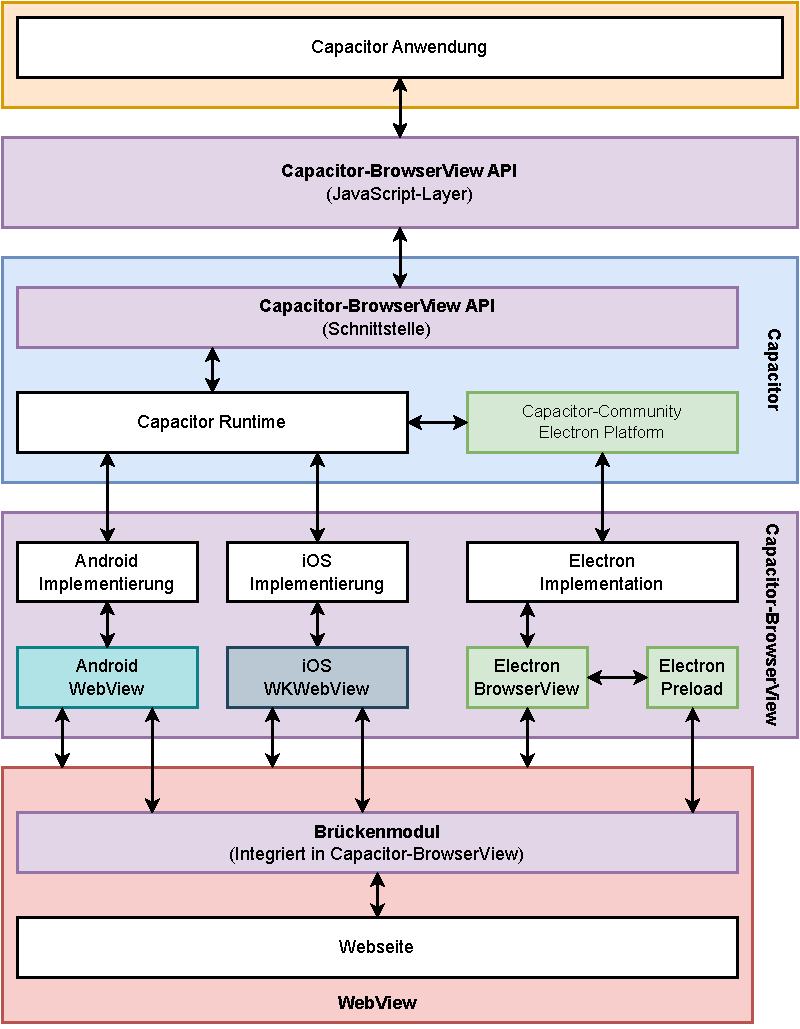
\includegraphics[width=\textwidth]{assets/03_Capacitor-BrowserView/03_Implementation.drawio.pdf}
    \caption[Capacitor-BrowserView / Implementierung]{Implementierung des Capacitor-BrowserView Plugins}
    \label{asset:Capacitor-BrowserView:Implementation}
\end{figure}

\newpage

\paragraph{Plugin API}

Das Capacitor-BrowserView Plugin erweitert seine \ac{api} um einen zusätzlichen JavaScript"=Layer, der zusätzliche nicht-native Funktionen wie das Entfernen bestimmter oder aller Event-Listener einer konkreten BrowserView implementiert.

Der JavaScript"=Layer ermöglicht auch die Erstellung von \enquote{BrowserView}"=Instanzen, indem die Plugin \ac{api} in eine Klasse gekapselt wird.
BrowserViews können dadurch einfach über eine Instanz dieser Klasse erstellt werden.
Dies vereinfacht die Verwendung der Plugin \ac{api} wesentlich, da Methoden für eine bestimmte BrowserView direkt von der entsprechenden Instanz ausgeführt werden können.
Anderenfalls müssten die Methoden mit der entsprechenden \acs{uuid} der BrowserView aufgerufen werden.

Ein weiterer Vorteil dieser Umsetzung ist eine Reduzierung der Fehleranfälligkeit, da die \acsp{uuid} der verwendeten BrowserViews nicht manuell verwaltet werden müssen.

\newpage

\paragraph{Implementierungen}

Um die Implementierung des Plugins auf allen Plattformen übersichtlich und wartungsfreundlich zu gestalten, sind sie in ihrer Struktur sehr ähnlich.
Sie bestehen jeweils aus zwei Teilen:

\begin{enumerate}
    \item Der erste Teil wird von der Capacitor Runtime aufgerufen. Er implementiert die \acs{api}-Struktur und wertet die Parameter der Methoden aus.
    \item Der zweite Teil implementiert die tatsächlichen Funktionen, wie das Erstellen und Steuern von WebViews sowie das Senden und Empfangen von Nachrichten zwischen der Capacitor Anwendung und den geladenen Webinhalten.
\end{enumerate}

Für die Implementierung des Plugins wurden ausschließlich die jeweiligen Plattform"=\acsp{api} verwendet, da WebViews auf jeder Plattform nativ unterstützt werden.
\cite{android:api, ios:api, electron}

\begin{note}
    Die offizielle Entwicklungsumgebung für iOS, Xcode, ist ausschließlich für macOS verfügbar.~\cite{xcode:support}
    Da während der Entwicklung nur Windows- und Linux-Geräte zur Verfügung standen, war das Implementieren und Testen des Plugins für iOS nicht möglich.
\end{note}

Die WebView \acsp{api} sind auf den verschiedenen Plattformen nicht vollständig identisch.~\cite{android:api, electron}
Daher musste für die Implementierung des Plugins ein Kompromiss gefunden werden. Einige fehlende Funktionen wurden im Plugin nachgebaut, und einige Funktionen werden aufgrund großer Unterschiede nicht unterstützt.

\begin{itemize}
    \setlength\itemsep{-0.5em}
    \item Um die Position einer WebViews unter Android festzulegen, muss die Pixeldichte des Geräts berücksichtigt werden. Andernfalls stimmen die Koordinaten und Abmessungen der WebView nicht mit der Capacitor Anwendung überein. Auch die Höhe der Statusleiste muss berücksichtigt werden, da sich die WebView sonst mit ihr überschneiden würde.
    \item Die Android WebView bietet eine Einstellung, um das Öffnen von Webinhalten in einem neuen Fenster zu erlauben oder zu verbieten.~\cite{android:api} Diese Funktion wurde für Electron nachträglich in das Plugin implementiert.
    \item Favicons von Webinhalten werden in der Android WebView direkt in einem Binärformat bereitgestellt, während in Electron nur der Link zum Icon bereitgestellt wird.~\cite{android:api, electron} Daher wird es vom Plugin nachträglich heruntergeladen. Um zudem eine einheitliche Interpretation des Favicons zu gewährleisten, wird es vom Plugin in Base64 kodiert.
    \item Android WebViews unterstützen standardmäßig keinen Vollbildmodus. Daher wurde diese Funktion nachträglich in das Plugin implementiert. Notwendige Parameter für einen vollständigen Vollbildmodus wurden von StackOverflow bezogen. \cite{android:api, stackoverflow}
\end{itemize}

\newpage

\paragraph{Interprozesskommunikation}

Um die Kommunikation zwischen geladenen Webinhalten, der Plugin Implementierung und der Capacitor Anwendung zu ermöglichen, wird unter Android die \fn{JavascriptInterface}"=\acs{api} der WebView verwendet.
Diese \ac{api} ermöglicht es, eine Java-Funktion in die Webseite einzuspeisen.~\cite{android:api}

Unter Electron wurde für ein ähnliches Verhalten das \fn{preload-script} mit der \fn{contextBridge}"=\acs{api} verwendet.
Diese \ac{api} ermöglicht es ebenfalls, eine Funktion in die Webseite einzuspeisen.~\cite{electron}

Die eingespeiste Funktion dient als Schnittstelle, um Daten von der geladenen Webseite an das Capacitor-BrowserView Plugin zu senden.
Das Plugin leitet dann die empfangenen Daten an die Capacitor Anwendung weiter.

Um Daten von der Capacitor Anwendung an die Webseite zu senden, verwendet das Plugin die \fn{evaluateJavascript}"=Methode der Android WebView bzw.\ die \fn{executeJavaScript}"=Methode der Electron BrowserView.
Dadurch kann ein JavaScript-Code auf der Webseite ausgeführt werden~\cite{android:api, electron}, der die Daten über die \fn{dispatchEvent} Web-\acs{api} an die entsprechenden Event-Listener auf der Webseite verteilt.

Zur Verbesserung der Benutzerfreundlichkeit wurde ein Brückenmodul entwickelt, welches eine vereinfachte \ac{api} für die Kommunikation zur Capacitor Anwendung auf der Webseite bereitstellt.
Das Modul übernimmt den Zugriff auf die eingespeiste Funktion \textit{(um Daten zu senden)}, die Registrierung von Event-Listener \textit{(um Daten zu empfangen)} sowie die Serialisierung und Deserialisierung der Nutzdaten mittels \ac{json}.

Um das automatische Laden des Brückenmoduls zu ermöglichen, wird das Modul beim Start des Ladevorgangs der Webseite ausgeführt.

Unter Electron ist das ausführen des Moduls jedoch erst erlaubt, wenn die Webseite vollständig geladen wurde.~\cite{electron}
Folglich könnte die Webseite nicht rechtzeitig auf die \ac{api} des Brückenmoduls zugreifen.
Um dennoch das rechtzeitige Laden des Moduls zu ermöglichen, wird das Electron \fn{preload-script} mit der \fn{contextBridge}"=\acs{api} verwendet.

\printfn
